\documentclass[a4paper]{scrartcl}
\usepackage{defaultstyle}
\usepackage{localstyle}

\title{Authorization Logic for App Policies}
\subtitle{Second Year Report}
\author{Joseph Hallett}
\date\today

\begin{document}
\maketitle

\begin{abstract}
  This report describes work done in the second year of the PhD.
  I give a brief overview of the topic; before describing the work completed this year.
  I also review what topics suggested in the thesis proposal.
  Work reimplementinging AppPAL, exploring store and user policies and looking at protocols for app distribution is described.
  I say what I expect to explore in the final year.
  Finally, I give a table of contents for the proposed thesis.
\end{abstract}

\section{Introduction}

Mobile devices let users pick the apps they want to run.
App stores offer a wide range of software for users to choose.
Users pick particular apps for a variety of reasons:
  ordering in the store~\citep{Prata:2012in},
  reviews and privacy concerns~\citep{Kelley:2013kc},
  and security rules from their employer.

Finding the right apps can be tricky:
  users need to work out which apps are well written, which are not going to abuse their data, which ones will work in the way they want
  and to find the apps which suit how they want to use their device.
This can be difficult as it isn't obvious how apps use the data each has access to.

People fall into patterns when thinking about the privacy issues around apps~\citep{Sadeh:2014vq}.
By capturing these patterns explicitly as policies they can be enforced automatically.
This reduces the burden on users to decide which apps they want.
Security-savvy users may design policies themselves: these could be shared with others or used in organisation-wide curated app stores.

Companies have policies about how phones should be used by employees.
With \emph{bring your own device} schemes employees use their personal devices for work.
IT departments in these companies may need to create policies so that the devices can be used securely with company information.
Ensuring compliance is often left to the employees.
By using an authorization logic I believe these policies can be enforced automatically.
This reduces the burden on users to ensure compliance, and IT departments to check it.

\section{Summary of second year work}

%\subsection{What I said I'd do}

In the thesis proposal I proposed primarily looking at the role of app stores this year.
Specifically I wanted to understand how users interacted with the stores.
This would enable us to better understand user behavior.
By better understanding user behavior I could write policies that described the users.
I said that I would:

\begin{itemize}
  \item Implement an app store filtered by AppPAL policies.
  \item Look at how users interact with apps, and the kinds of policies they apply, as well as what happens when their policies change.
  \item Look at how the policies vary within categories of apps.
  \item Explore how policies could be composed and joined.
  \item Explore what happens when policies are attacked.
\end{itemize}

Several of these topics seemed to change as year went on.
I implemented a system for creating app stores based on an AppPAL policy, but when I also gained access to real installation data.
Using this data I started to look at what apps users pick from stores and the kinds of policies they apply.
I started looking at greater detail at the distribution mechanisms and policies within app stores.

Some existing work continued on from the first year.
The initial prototype of SecPAL became unweildy, wouldn't run on Android, and I found major bugs in the implementation.
I reimplemented it, renamed it AppPAL, and have been optimizing and improving it throughout the year.
Other work was started from necessity.
I wanted a means of systematically running tools over large numbers of apps and collecting the results;
  so I built one and have used the data collected from it in other aspects of the project.

In the next few sections I describe some of the work I have completed in the second year; and show some of the findings.

\subsection{Reimplemented AppPAL in Java.}

The prototype started in the first year had several bugs, relating to policy checking, in it and became unweildy to fix.
Because of lack of compiler support the Haskell implementation could not run on Android, making on device experimentation harder.
I reimplemented it in Java and made sure it was portable, running a library in an app, or Java program.
The current implementation contains roughly the same number of lines of code, but runs everywhere and is significantly easier to modify.

The performance of the library when searching an assertion context is reasonable.
Performance using synthetic benchmarks designed to test the search procedure is reasonable.
The search procedure is at its slowest when performing large repeated delegations.
I designed two synthetic benchmarks to check that the search procedure performed acceptably.
The \emph{straight} benchmark consists of a single long chain of delegation.
The \emph{forking} benchmark consists of a binary tree of principals delegating to each other.
These benchmarks are reasonable as they model the worst kinds of policies (though worse ones could of course be designed).

Cn a Nexus 4 device checking times are measured in seconds when there are hundreds of delegations in a single policy check, and in minutes when there are thousands (\autoref{fig:benchmarks}).
When describing hypothetical real policies, I typically only have a few delegations, and not long delegation chains, so I believe the performance will is acceptable.
I believe that the AppPAL constraints will be the slowest part of checking a policy.
Since they can execute arbitrary programs or include network requests their performance is independent of AppPAL.
In practice the only ones I have used (so far) are permissions checks which are very fast.
Slowly evaluating constarints could be used but this may lead to policy design decisions to limit the number of constraints in policies.
Current practical policies check five or six permissions per app.
Since the numbers of checks are small it is not worth optimizing currently.

\begin{figure}
  \begin{minipage}{0.49\linewidth}
    \footnotesize
    \begin{tabular}{cccc}
       \toprule
       Policy   & Principals & Parse (s) & Check (s) \\
       \midrule
       Straight & 10    & 0.01      & 0.04      \\
       Straight & 100   & 0.05      & 1.00      \\
       Straight & 500   & 0.32      & 21.07     \\
       Straight & 1000  & 0.43      & 87.75     \\
       \midrule
       Forking  & 256   & 0.10      & 1.93      \\
       Forking  & 512   & 0.23      & 7.47      \\
       Forking  & 1024  & 0.45      & 28.29     \\
       Forking  & 2048  & 0.85      & 117.68    \\
       \bottomrule
    \end{tabular}
  \end{minipage}
  \begin{minipage}{0.49\linewidth}
    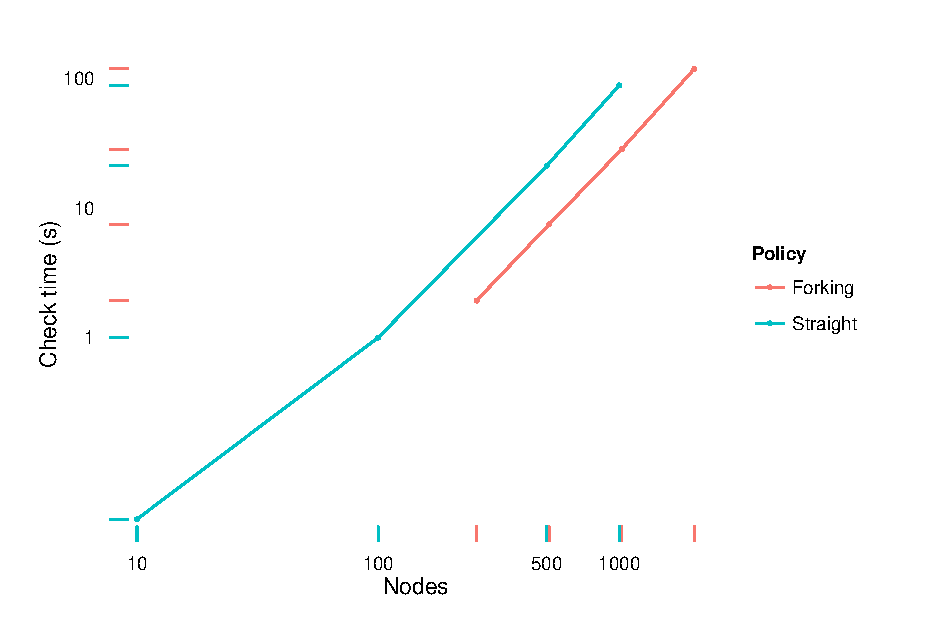
\includegraphics[width=\linewidth]{./images/benchmarks.eps}
  \end{minipage}
  \caption{Benchmarking results on a Nexus 4 Android phone.}
  \label{fig:benchmarks}
\end{figure}

\subsection{Built a \ac{SKB} exporting statements to AppPAL.}

As part of the AppPAL framework I imagined using results from static analysis tools as constraints within the language.
To collect and store these results I built an extensible \ac{SKB} that was lightweight and which could be trivially extended.
Implemented in Ruby the \ac{SKB} supports running metadata-fetching and static-analysis tools in parallel over large collection of apps.
Adding tools is quick and painless (add a library to Ruby, or a file to a configuration folder implementing a class interface).
The \ac{SKB} exports statements to AppPAL, and holds around 40,000 apps at the moment.

\subsection{Explored existing app store privacy policies.}

There are many Android app stores available.
I believed that each of the different stores would have different policies for kinds of apps, developers, and privacy conditions.
I read the privacy, developer and user policies for four different app stores (Google Play, Amazon, Aptoide and Yandex) to compare them.
In practice I found that the policies tended to be very similar; perhaps even copied in some places.
There were some differences when it came to payment processing, and minimum ages to use the store.
Some stores (excepting Google's) kept some right to modify any apps, typically for advertising.
This might form the basis of interesting trust relationships as the app would need to be resigned by the store to be installed.
Resigning is interesting because the trust in the authenticity of the app moves from the developer to the store.
A summary of some of the different terms and conditions is shown in \autoref{tab:terms}.

\begin{figure}[!h]\tiny
\begin{tabulary}{\linewidth}{lLLLL}
\toprule
                     & Google Play                                                                                                                                                        & Amazon & Yandex & Aptoide \\
\midrule
User ID              & Name address and billing details.
                     & Amazon ID.
                     & None for free apps, payment details for paid.
                     & Contact details. No verification but agreement not to lie.                                                                                                        \\ \addlinespace
Client info taken    & Installation data, device ID, browsing history, cookies. Can opt out.
                     & Device ID, network info, location, usage data.
                     & Device ID, SIM number, Device content, System data, browsing history.
                     & Transaction history.  They may share it with developers.                                                                                                          \\ \addlinespace
Customer Payments    & Google Wallet and others at Google's discretion.
                     & Amazon.
                     & Approved processor by Yandex or store operator.
                     & Approved processor by Aptoide.                                                                                                                                    \\ \addlinespace
Who is paid?         & Google Commerce.
                     & Amazon.
                     & Developer.
                     & Store owner.                                                                                                                                                      \\ \addlinespace
Prices set by        & Developer.
                     & Amazon.
                     & Developer (but Yandex may restrict to set values).
                     & Developer and store owner.                                                                                                                                        \\ \addlinespace
Refunds              & Only for defective or removed content. A refund may be requested for two hours after purchase.
                     & No.
                     & Upto 15 minutes after purchase. No for IAP.
                     & Upto 24 hours after purchase.                                                                                                                                     \\ \addlinespace
Age of use           & At least 13.
                     & Any age (with consent of guardian).  No alcohol related content bellow 21.
                     & At least 14.
                     & A legal age to form a contract with Aptoide.                                                                                                                      \\ \addlinespace
Update provision     & You agree to receive updates.
                     & By default.
                     & Yes for security and bugfixes.
                     & Yes agree to receive updates.                                                                                                                                     \\ \addlinespace
Moderation           & No obligation (but they may).
                     & Publisher obliged to provide info which may be used to give ratings.  Amazon will not check these ratings are accurate.
                     & No obligation (but they may).
                     & No obligation (but they may).  Trusted app mark does not indicate moderation.                                                                                     \\ \addlinespace
Acceptable use       & No use as part of a public performance, or for dangerous activities where failure may lead to death.
                     &
                     &
                     & No modification, rental, distribution or derivative works.  You may use the software.                                                                             \\ \addlinespace
Store rights to app  & Marketting and optimizing Android.
                     & Distribution, evaluation, modification, advertising, and creating derivatives for promotion.
                     & Advertising.
                     & Modification and re-selling.                                                                                                                                      \\ \addlinespace
Withdrawl from sale  & Immediate.
                     & 10 days, or 5 days if for copywrite reasons.
                     & 90 days. A copy will be retained.
                     & You may.                                                                                                                                                          \\ \addlinespace
Developer ID         & Google account and billing details.
                     & Amazon ID.
                     & Email, company name, tax-id.
                     & Email (preferably a Google developer one).                                                                                                                        \\ \addlinespace
EULA                 & Default offered.
                     & Only if it doesn't interfere with Amazon's terms.
                     & Must be provided.
                     & Default offered                                                                                                                                                   \\ \addlinespace
Content restrictions & No alternate stores, sexual, violence, IP infringing, PII publishing, illegal, gambling, malware, self-modifying or system modifying content.  No unpredictible network use.
                     & No offensive, pornography, illegal, IP infringing or gambling content.
                     & No defects. No illegal, disrutpive, sexual, IP infinging, PII stealing, alternative stores, or open-source content.
                     & No displaying or linking to illegal, privacy interfering, violent, PII stealing, IP infringing content.  Nothing \emph{spammy} or with unpredictable network use. \\ \addlinespace
Payout rates         & 70\% of user's payment.
                     & 70\% list price (minus card fees).
                     & 70\% net-revenue (minus card fees).
                     & 75\% revenue share (minus card fees).                                                                                                                             \\ \addlinespace
\bottomrule
\end{tabulary}
\caption{Summary of conditions in different stores.}
\label{tab:terms}
\end{figure}

\subsection{Explored distribution mechanisms in existing stores.}

A user buying an app probably wants the app sent to their device.
Using an SSL proxy I started looking at the precise distribution mechanisms and started reverse engineering their protocols.
For simple website stores, such as Opera's mobile store, where apps are distributed without encryption, it is trivial to modify downloaded apps on the fly.
Various security flaws were found.
Amazon's store was the only one to enable certificate pinning but this was only for the logon process, after which the SSL proxy worked fine.
Google's store occasionally seemed to drop encryption when downloading APK files, allowing a listener to identify the apps someone used; though this seemed to stop happening a month later.
Working from the network traffic and by reverse engineering the store I attempted to create an abstract description of the protocol used to buy apps (\autoref{fig:protocol}).

I would like to continue this work into the next year.
Each of the stores I looked at had a slightly different protocol for buying apps and a different means of downloading them onto the device.
I might imagine in an AppPAL-enhanced app store apps being supplied with some assertions about their behavior.
Working out how to include these in the download protocols, (and with knowledge distribution in general, proposed in \autoref{ssec:kdp}) seems interesting.

\begin{figure}[!h]
  \begin{minipage}{0.48\linewidth}
    \begin{center}
    \begin{tabular}{rrc}
      \toprule
      1. & $C \longrightarrow S$:        & $U, C, a_{\text{d}} $  \\ \addlinespace
      2. & $S \longrightarrow C$:        & $a_{\text{d}}, ? $     \\ \addlinespace
      3. & $C \longrightarrow S$:        & $U, ! $                \\ \addlinespace
      4. & $S \longrightarrow C$:        & $a_{\text{d}}, \$ $    \\ \addlinespace
      5. & $C \longrightarrow S$:        & $U, a_{\text{d}}, \$ $ \\ \addlinespace
      6. & $S \longrightarrow C$:        & $S^\prime$             \\ \addlinespace
      7. & $C \longrightarrow S^\prime$: &                        \\ \addlinespace
      8. & $S^\prime \longrightarrow C$: & $a$                    \\
      \bottomrule
    \end{tabular}
  \end{center}

    {\footnotesize In message 6, $S$ redirects $C$ using a 302-redirect message.
      By replaying message 7 I found I could redownload the app on a different client.
      I found that the redirection to the other server sometimes did not use SSL.}
  \end{minipage}
  \begin{minipage}{0.48\linewidth}
    \begin{tabulary}{\linewidth}{cC}
      \toprule
      Symbol         & Meaning                                                           \\
      \midrule
      $S$            & Store (\texttt{android.clients.google.com}).                      \\
      $C$            & Client the app store app running on the phone.                    \\
      $U$            & User, identified by a token.                                      \\
      $a$            & An app.                                                           \\
      $a_{\text{d}}$ & a description of the app $a$.                                     \\
      $?$            & Purchase challenge                                                \\
      $!$            & Purchase challenge responce (seemingly derived from $?$ and $U$). \\
      $\$$           & Download token.                                                   \\
      $S^\prime$     & Alternate store URL                                               \\
      \bottomrule
    \end{tabulary}
  \end{minipage}
  \caption{Abstraction of the protocol used by Google's Play store to purchase an app.}
  \label{fig:protocol}
\end{figure}

\subsection{User app installation behaviour}

Mobile device users have policies about what data apps should be able to collected.
Lin~\etal~\citep{Sadeh:2014vq} identified four different privacy policies when users think about apps; however they did not look at whether they enforced them in practice.
Using AppPAL I implemented a simplification of the policies Lin~\etal identified.
The Carat project~\citep{Oliner:2013ht} collected app installation data from users who installed their energy tracking app.
They shared this data with us in an anonymised form where I could see who had installed what provided I knew the package names of the apps they installed.
Ignoring system apps, using the \ac{SKB} I deannonimized 4,300 apps (5\%) which accounted for 50\% of all app installs.
I selected 44,000 users for whom I knew 20 or more app installs.

Using the Carat data I measured the extent each user conformed with the privacy policies.
I also took a list of known malware and \ac{PUP} software from McAfee to measure the extent of malware installations on Android.
From this I tested whether users who enforce their privacy policies install less malware.

I found that very few users follow these policies, but a few users who do seem to be installing apps meeting these policies most of the time (\autoref{sfig:lin}).
For the unconcerned policy (the most permissive) only 1,606 users (4\%) had 50\% compliance;
and only 120 users (0.3\%) had 80\% compliance.
For the stricter conservative policy only 60 users were complying half the time, and just 7 more than 80\% of the time.
This suggests that while users may have privacy preferences the majority are not attempting to enforce them.

I found 1\% of the users had a PUP or malicious app installed (\autoref{sfig:malware}).
A user is 3 times more likely to have a PUP installed than malware.
Only 9 users had both a PUP and malware installed.
Users who were complying more than half the time with the conservative or advanced policies complied with the malware or PUP policies fully (\autoref{sfig:compare}).
This is significant (P-value $< 0.05$) and suggests that users who pick their apps carefully are less likely to experience malware.

\begin{figure}\centering
  \begin{subfigure}[b]{0.48\linewidth}
    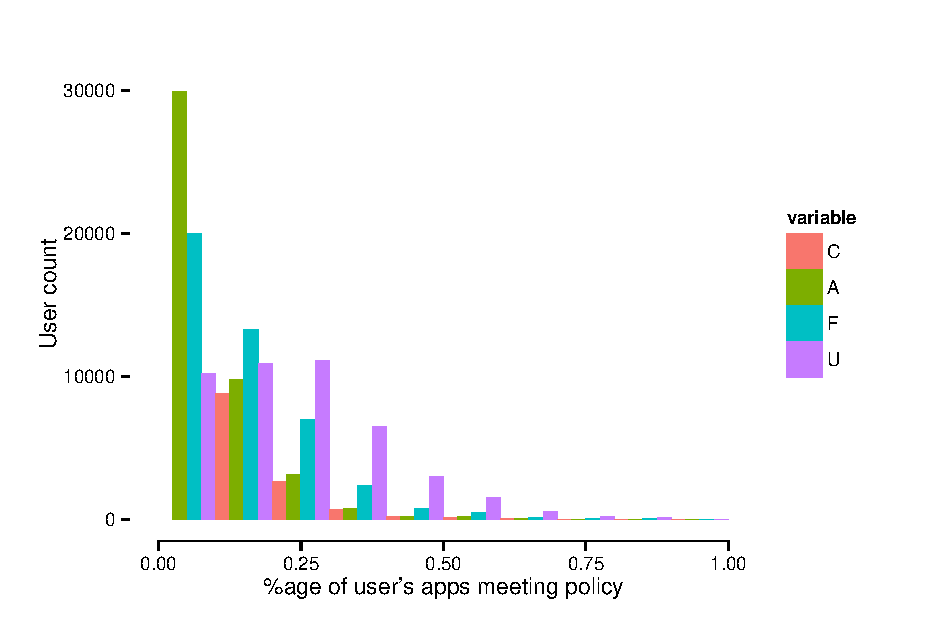
\includegraphics[width=\linewidth]{./images/lin-2yr.eps}
    \caption{User conformance to identified privacy policies.}
    \label{sfig:lin}
  \end{subfigure}
  \begin{subfigure}[b]{0.48\linewidth}
    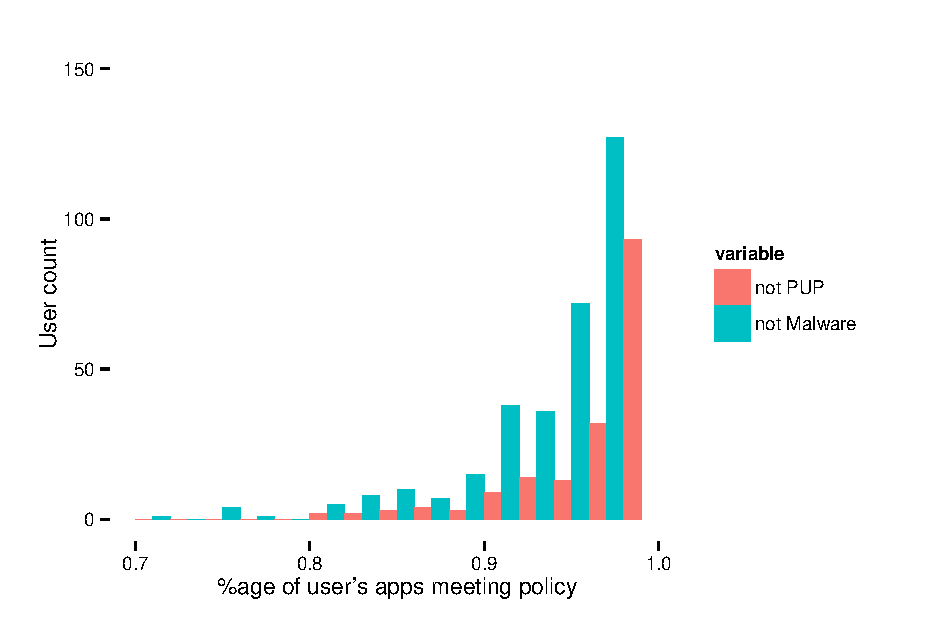
\includegraphics[width=\linewidth]{./images/malware-2yr.eps}
    \caption{User malware installation rates.}
    \label{sfig:malware}
  \end{subfigure}

  \begin{subfigure}[b]{\linewidth}
    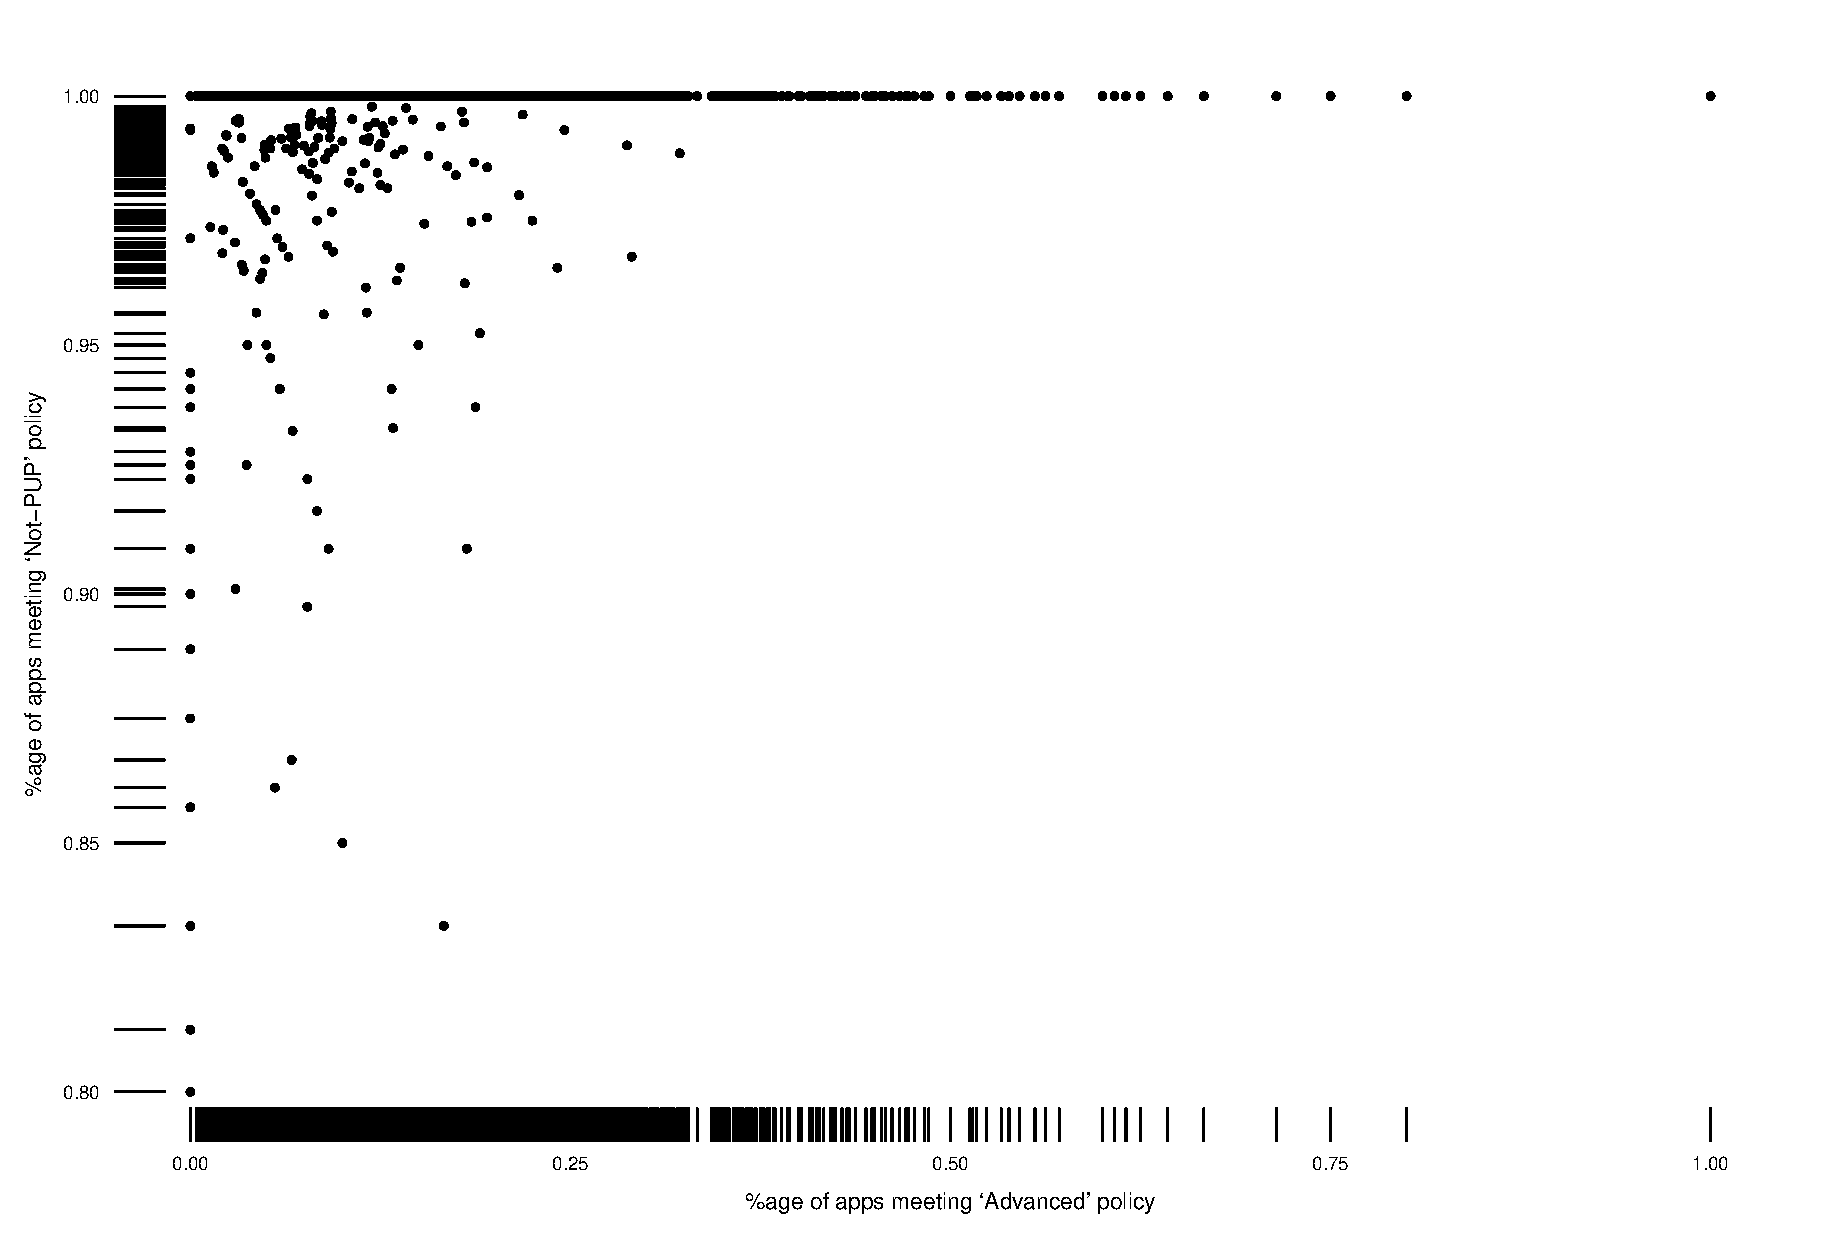
\includegraphics[width=\linewidth]{./images/compare-2yr.eps}
    \caption{Comparison of users following the advanced policy with malware installation.}
    \label{sfig:compare}
  \end{subfigure}

  \caption{Results from study on user app installation behaviour.}
  \label{fig:lin}
\end{figure}

This work was presented as a poster at SOUPS~\citep{Hallett:2015ty}, and I are aiming to publish it fully as part of a paper targetting the ESSoS conference (a draft of which is attached as an appendix).

\section{Next directions}

In the thesis proposal I suggested that in the third year I might look at advanced kinds of policies.
I also wanted to look at what might happen when policies have to deal with updates, to policies and apps on the device.
Some included:
\begin{itemize}
  \item The app collusion problem.
  \item What happens when policies are composed?
  \item Policy revocation and modification.
  \item App update policies.
\end{itemize}

Some of these problems have become less interesting: for example app updates
Various different policies for updates could be encoded in AppPAL for the precise behaviour of an update.
Since most stores mandate accepting updates in the user agreement, however, and the default behavior is to autoinstall updates it has become somewhat irreleveant.
Updates typically include bugfixes so it is in the user's interests to accept them (despite what they may believe~\citep{Vaniea:2014fk}).
Implementing methods to weaken security does not seem to be worthwhile.
That said using AppPAL as a modelling language to precisely describe the trust mechanisms and delegations in an update is interesting and I might continue in that direction.

Likewise, policy modification is not interesting.
Apps should be rechecked before they can be allowed to run again.
If they now break the policy, the user should be prompted to remove the app or make an exception.
Results from long-running static analysis tools can be stored by the \ac{SKB}.
These could be reused by AppPALs constraint mechanisms to avoid recomputation, if no other changes were made.

The app collusion problem is still interesting.
Whilst it is concievable that AppPAL policies could describe and prevent attacks, to actually implement the protection in a way that could be used would probably require modifications to the intent system, and potentially binder (Android's primary IPC mechanism) and this probably makes it out of scope of the PhD.

The mechanisms for mechanically composing policies in AppPAL are trivial\footnote{\lstinline{'user' says 'composed-policy' isMetBy(App)  if 'pol1' isMetBy(App), 'pol2' isMetBy(App).}} but what might happen when two principals actively disagree is more interesting.
AppPAL doesn't have support for negation, but it feels right that there should be some way to distinguish between a principal saying an app meets, does not meet, or does not know whether it meets a policy.
Continuing research should continue along with the protocols for distributing AppPAL statements.

\subsection{Knowledge distribution protocol}
\label{ssec:kdp}

I have a means of enforcing policies and I have started looking at the kinds of policies users might want to use.
When describing AppPAL policies I have thought about delegation relationships and how different principals can be trusted to help make decisions.
What isn't necessarily clear is how these principals get to make these statements and how they are transferred from speaker to speaker.

On a memory constrained device, like a mobile phone, storing a database of all possible ground AppPAL statements by every speaker is clearly not viable.
There are almost 1.5 million apps available on the Google Play store, not including other stores or multiple versions of the same app.
Storing data on all apps will not work.
In the papers on SecPAL~\citep{Becker:2006vh,Becker:2009vt} (on which AppPAL is based) there is little talk about how the knowledge should be distributed.
They describe how principals should sign their AppPAL statements to identify themselves as having said them, and how an X.509-style public key system could be used to tie keys to principals.  This tells us how to check the statements are not forged but doesn't give the distribution mechanisms.
Related languages~\citep{Becker:2009ula,Aziz:2011vt,Gurevich:2008fz,Gurevich:Qo5E3M3} extended SecPAL language features but also didn't specify the distribution protocol.
SecPAL was designed to be a distributed language with principals delegating statements.
Without a distribution protocols some scenarios can become difficult.

One time these problems may occur is when
Alice wants to install an app on her phone.
Her installation policy requires confirmation the app is not malware.
She knows that McAfee can say (possibly with further delegation) whether an app is malicious or not;
  but this is a new app and she does not have any prior information about it.
She needs to get more information.
This scenario raises more questions:

\begin{itemize}
  \item How does she ask McAfee about the app?  What is the protocol for speaking and distributing statements?
  \item If the app is really new McAfee may not know about it either. How should she send it to them for analysis?  What should she do while she waits: keep waiting, fail and keep a note to recheck later or fail and never ask again about the app?  Are there legal issues surrounding Alice redistributing the app to McAfee?
  \item How do McAfee respond?  AppPAL does not contain negation but in this scenario it would be helpful to distinguish a statement from McAfee that the app is safe, from one where they know it is definitely malware, from one where they are unsure and wish to err on the side of caution and not make a definite statement.
  \item If McAfee wish to delegate the decision they could issue another \emph{can-say} statement.   Should McAfee send the public key and any statements from the delegated party to the user, or just the server address and a reference to the public key on a PKI server?
  \item When should Alice ask McAfee?  Before any evaluation would be the easiest time as it would require no change to the evaluation algorithm but during the evaluation might be more appropriate as statements could be imported as needed.
\end{itemize}

Work this year should look at developing a strategy, and defining a protocol to share and acquire knowledge through AppPAL statements on demand.
This would be a worthwhile contribution, as it is novel, and would help extend AppPAL from a SecPAL instantiation to it's own language.


\subsection{Case study}

Having an authorization logic model and enforce a real world policy shows the limitations and expressivity of a language.
It also shows that it is applicable to current compliance problems and solves \emph{real world problems} rather than just the policies I have learnt from user behaviour.

A natural source of these real world policies is corporate \ac{BYOD} policies, where employers describe restrictions on the useage of mobile devices in the workplace.
The \ac{NIST} have published recomendations for mobile device security and \ac{BYOD} in the workplace~\citep{Souppaya:2013jf,Scarfone:2009vy}.
Translating the mobile device relevant sections into AppPAL and showing their enforcement might make a good case study.
The study would focus on any difficulties in translating the policies and the extent the policy could be enforced automatically.

AppPAL policies I have used so far have been synthetic.
This has been fine for testing and demonstrating the language, but a larger example drawn from a real policy would help give AppPAL credibility.


\section{Proposed thesis outline}

\begin{quote}
  \emph{Hypothesis.} Automatic tools and policy languages would provide a
  better means of enforcement for mobile device policies than existing
  mechanisms which rely on manual inspection.
\end{quote}

\begin{enumerate}
  \item Introduction
  \item Mobile ecosystems
    \begin{description}
      \item[App stores and mobile app deployment]
        \hfill
        \begin{itemize}
          \item Introduce app stores and current development practices.
          \item Show the differences between different market places and the platforms (iOS vs Android).
        \end{itemize}
      \item[Android Security Model]
        \hfill
        \begin{itemize}
          \item Introduce the android permissions model and how different apps can access functionality provided by the platform.
          \item Show how app signing works.
        \end{itemize}
      \item[Android policies]
        \hfill
        \begin{itemize}
          \item Introduce the need for policies and the motivation for the PhD.
          \item Show how users do not seem to be following their privacy policies.
          \item Explain how some companies have mobile device policies, and how users are frustrated with data leaks.
          \item Show existing tools, such as Kirin, and explain why they're not good enough.
        \end{itemize}
    \end{description}
  \item AppPAL
    \begin{description}
      \item[The need for a policy language]
        \hfill
        \begin{itemize}
          \item Introduce scenarios where AppPAL can be used to enforce a policy
          \item Show trust relationships between different principals (a user at work).
          \item Start to introduce the language.
        \end{itemize}
      \item[Design and implementation of AppPAL]
        \hfill
        \begin{itemize}
          \item Formally present the language, as an instantiation of SecPAL.
          \item Show evaluation algorithm.
        \end{itemize}
      \item[Deployment]
        \hfill
        \begin{itemize}
          \item Show applications using AppPAL.
          \item Stores generated by policy.
          \item On device policy checking.
          \item Device configuration by policy (if I can get access to Android M features)
        \end{itemize}
      \item[Distribution]
        \hfill
        \begin{itemize}
          \item Define protocol for knowledge acquisition.
          \item Describe implementation of protocol.
        \end{itemize}
    \end{description}
  \item Evaluation
    \begin{description}
      \item[Case study]
        \hfill
        \begin{itemize}
          \item Show how I can take a corporate policy and enforce it using AppPAL.
          \item Show the language is expressive enough to describe real policy scenarios.
          \item Show it works in \emph{the real world}.
        \end{itemize}
    \end{description}
  \item Related work
  \item Future work
\end{enumerate}

\bibliography{report}

\newpage
\appendix

\section{Paper for ESSoS 2016}

The attached paper is a draft being prepared for the ESSoS\footnote{Engineering Secure Software and Systems} symposium.
The paper will introduce the AppPAL language and its implementation.
I give sanity checking benchmarks to show its performance is not unreasonable.
Finally I demonstrate AppPAL by presenting our work using AppPAL to filter user's privacy policies from our SOUPS poster, as part of a full paper.

\includepdf[pages=-]{../essos-2016-apppal/paper.pdf}


\end{document}

